%% abtex2-modelo-trabalho-academico.tex, v-1.9 laurocesar
%% Copyright 2012-2013 by abnTeX2 group at http://abntex2.googlecode.com/ 
%%
%% This work may be distributed and/or modified under the
%% conditions of the LaTeX Project Public License, either version 1.3
%% of this license or (at your option) any later version.
%% The latest version of this license is in
%%   http://www.latex-project.org/lppl.txt
%% and version 1.3 or later is part of all distributions of LaTeX
%% version 2005/12/01 or later.
%%
%% This work has the LPPL maintenance status `maintained'.
%% 
%% The Current Maintainer of this work is the abnTeX2 team, led
%% by Lauro César Araujo. Further information are available on 
%% http://abntex2.googlecode.com/
%%
%% This work consists of the files abntex2-modelo-trabalho-academico.tex,
%% abntex2-modelo-include-comandos and abntex2-modelo-references.bib
%%

% ------------------------------------------------------------------------
% ------------------------------------------------------------------------
% abnTeX2: Modelo de Trabalho Academico (tese de doutorado, dissertacao de
% mestrado e trabalhos monograficos em geral) em conformidade com 
% ABNT NBR 14724:2011: Informacao e documentacao - Trabalhos academicos -
% Apresentacao
% ------------------------------------------------------------------------
% ------------------------------------------------------------------------

\documentclass[
	% -- opções da classe memoir --
	12pt,				% tamanho da fonte
	openright,			% capítulos começam em pág ímpar (insere página vazia caso preciso)
	oneside,			% para impressão em verso e anverso. Oposto a oneside
	a4paper,			% tamanho do papel. 
	% -- opções da classe abntex2 --
	chapter=TITLE,		% títulos de capítulos convertidos em letras maiúsculas
	section=TITLE,		% títulos de seções convertidos em letras maiúsculas
	%subsection=TITLE,	% títulos de subseções convertidos em letras maiúsculas
	%subsubsection=TITLE,% títulos de subsubseções convertidos em letras maiúsculas
	% -- opções do pacote babel --
	english,			% idioma adicional para hifenização
	%french,				% idioma adicional para hifenização
	%spanish,			% idioma adicional para hifenização
	brazil				% o último idioma é o principal do documento
	]{abntex2}

% ---
% PACOTES
% ---

% ---
% Pacotes fundamentais 
% ---
\usepackage{lmodern}			% Usa a fonte Latin Modern			
\usepackage[T1]{fontenc}		% Selecao de codigos de fonte.
%\usepackage[utf8]{inputenc}		% Codificacao do documento (conversão automática dos acentos)
\usepackage{lastpage}			% Usado pela Ficha catalográfica
\usepackage{indentfirst}		% Indenta o primeiro parágrafo de cada seção.
\usepackage{color}				% Controle das cores
\usepackage{graphicx}			% Inclusão de gráficos
\usepackage{microtype} 			% para melhorias de justificação
% ---

\usepackage{listings}
\usepackage{booktabs} %Melhora o visual das tabelas
\usepackage{tabulary} %
\usepackage[table]{xcolor} %
		
% ---
% Pacotes adicionais, usados apenas no âmbito do Modelo Canônico do abnteX2
% ---
\usepackage{lipsum}				% para geração de dummy text
% ---

% ---
% Pacotes de citações
% ---
\usepackage[brazilian,hyperpageref]{backref}	 % Paginas com as citações na bibl
\usepackage[alf]{abntex2cite}	% Citações padrão ABNT

\usepackage{tikz}
\usetikzlibrary{calc,trees,positioning,arrows,chains,shapes.geometric,%
    decorations.pathreplacing,decorations.pathmorphing,shapes,%
    matrix,shapes.symbols}

\tikzset{
	>=stealth',
  punktchain/.style={
    rectangle, 
    rounded corners, 
    % fill=black!10,
    draw=black, very thick,
    text width=10em, 
    minimum height=3em, 
    text centered, 
    on chain},
  line/.style={draw, thick, <-},
  element/.style={
    tape,
    top color=white,
    bottom color=blue!50!black!60!,
    minimum width=8em,
    draw=blue!40!black!90, very thick,
    text width=10em, 
    minimum height=3.5em, 
    text centered, 
    on chain},
  every join/.style={->, thick,shorten >=1pt},
  decoration={brace},
  tuborg/.style={decorate},
  tubnode/.style={midway, right=2pt},
}

% --- 
% CONFIGURAÇÕES DE PACOTES
% --- 

% ---
% Configurações do pacote backref
% Usado sem a opção hyperpageref de backref
\renewcommand{\backrefpagesname}{Citado na(s) página(s):~}
% Texto padrão antes do número das páginas
\renewcommand{\backref}{}
% Define os textos da citação
\renewcommand*{\backrefalt}[4]{
	\ifcase #1 %
		Nenhuma citação no texto.%
	\or
		Citado na página #2.%
	\else
		Citado #1 vezes nas páginas #2.%
	\fi}%
% ---

% ---
% Informações de dados para CAPA e FOLHA DE ROSTO
% ---
\titulo{\textsc{Modelo de Banco de Dados para Gerenciamento de Pizzaria: Modelagem e Implementação}}
\autor{Guilherme Augusto de Macedo \and Matheus Liberato Domingues da Silva \and Victor Hugo Carlquist da Silva}
\local{Campos do Jordão}
\data{2013}
\orientador{Paulo Giovani de Faria Zeferino}
% \coorientador{Equipe \abnTeX}
\instituicao{Instituto Federal de Educação, Ciência e Tecnologia de São Paulo - \textit{campus} Campos do Jordão}
\tipotrabalho{Trabalho Final}
% O preambulo deve conter o tipo do trabalho, o objetivo, 
% o nome da instituição e a área de concentração 
\preambulo{Trabalho final apresentado na disciplina de Banco de Dados II no quarto módulo do curso de Tecnologia em Análise e Desenvolvimento de Sistemas do IFSP-CJO.}


% Configurações de aparência do PDF final

% alterando o aspecto da cor azul
\definecolor{blue}{RGB}{41,5,195}

% informações do PDF
\makeatletter
\hypersetup{
     	%pagebackref=true,
		pdftitle={\@title}, 
		pdfauthor={\@author},
    	pdfsubject={\imprimirpreambulo},
	    pdfcreator={LaTeX with abnTeX2},
		pdfkeywords={abnt}{latex}{abntex}{abntex2}{trabalho acadêmico}, 
		colorlinks=true,       		% false: boxed links; true: colored links
    	linkcolor=blue,          	% color of internal links
    	citecolor=blue,        		% color of links to bibliography
    	filecolor=magenta,      	% color of file links
		urlcolor=blue,
		bookmarksdepth=4
}
\makeatother
% --- 

% --- 
% Espaçamentos entre linhas e parágrafos 
% --- 

% O tamanho do parágrafo é dado por:
\setlength{\parindent}{1.3cm}

% Controle do espaçamento entre um parágrafo e outro:
\setlength{\parskip}{0.2cm}  % tente também \onelineskip

% ---
% compila o indice
% ---
\makeindex
% ---

\lstset{language=SQL,
	basicstyle = \ttfamily\footnotesize, % Tamanho da fonte do código
	numbers = left, % Posição da numeração das linhas
	numberstyle = \tiny\color{blue}, % Estilo da numeração de linhas
	stepnumber = 1, % Numeração das linhas ocorre a cada quantas linhas?
	numbersep = 10pt, % Distância entre a numeração das linhas e o código
	backgroundcolor = \color{white}, % Cor de fundo
	showspaces = false, % Exibe espaços com um sublinhado
	showstringspaces = false, % Sublinha espaços em Strings
	showtabs = false, % Exibe tabulação com um sublinhado
	frame = l, % Envolve o código com uma moldura, pode ser single ou trBL
	rulecolor = \color{black}, % Cor da moldura
	tabsize = 2, % Configura tabulação em x espaços
	captionpos = b, % Posição do título pode ser t (top) ou b (bottom)
	breaklines = true, % Configura quebra de linha automática
	breakatwhitespace= false, % Configura quebra de linha
	%title = \lstname, % Exibe o nome do arquivo incluido
	%caption = \lstname, % Também é possível usar caption no lugar de title
	keywordstyle = \color{blue}, % Estilo das palavras chaves
	commentstyle = \color{green}, % Estilo dos Comentários
	stringstyle = \color{red}, % Estilo de Strings
	escapeinside = {\%*}{*)}, % Permite adicionar comandos LaTeX dentro doseu có digo
	morekeywords ={*,USE,GO} % Se quiser adicionar mais palavras-chave
}

% ----
% Início do documento
% ----
\begin{document}

% Retira espaço extra obsoleto entre as frases.
\frenchspacing 

% ----------------------------------------------------------
% ELEMENTOS PRÉ-TEXTUAIS
% ----------------------------------------------------------
% \pretextual

% ---
% Capa
% ---
\imprimircapa
% ---

% ---
% Folha de rosto
% (o * indica que haverá a ficha bibliográfica)
% ---
\imprimirfolhaderosto*
% ---

% ---
% Inserir a ficha bibliografica
% ---

% Isto é um exemplo de Ficha Catalográfica, ou ``Dados internacionais de
% catalogação-na-publicação''. Você pode utilizar este modelo como referência. 
% Porém, provavelmente a biblioteca da sua universidade lhe fornecerá um PDF
% com a ficha catalográfica definitiva após a defesa do trabalho. Quando estiver
% com o documento, salve-o como PDF no diretório do seu projeto e substitua todo
% o conteúdo de implementação deste arquivo pelo comando abaixo:
%
% \begin{fichacatalografica}
%     \includepdf{fig_ficha_catalografica.pdf}
% \end{fichacatalografica}
\begin{fichacatalografica}
	\vspace*{\fill}					% Posição vertical
	\hrule							% Linha horizontal
	\begin{center}					% Minipage Centralizado
	\begin{minipage}[c]{12.5cm}		% Largura
	
	\imprimirautor
	
	\hspace{0.5cm} \imprimirtitulo  / \imprimirautor. --
	\imprimirlocal, \imprimirdata-
	
	\hspace{0.5cm} \pageref{LastPage} p. : il. (algumas color.) ; 30 cm.\\
	
	\hspace{0.5cm} \imprimirorientadorRotulo~\imprimirorientador\\
	
	\hspace{0.5cm}
	\parbox[t]{\textwidth}{\imprimirtipotrabalho~--~\imprimirinstituicao,
	\imprimirdata.}\\
	
	\hspace{0.5cm}
		1. Complexidade de Algoritmo.
		2. Processamento de Imagens.
		I. Autor.
		II. Título
		III. Orientador.
		IV. Faculdade.
		V. Título\\ 			
	
	\hspace{8.75cm} CDU 02:141:005.7\\
	
	\end{minipage}
	\end{center}
	\hrule
\end{fichacatalografica}
% ---


% ---
% Inserir folha de aprovação
% ---

% Isto é um exemplo de Folha de aprovação, elemento obrigatório da NBR
% 14724/2011 (seção 4.2.1.3). Você pode utilizar este modelo até a aprovação
% do trabalho. Após isso, substitua todo o conteúdo deste arquivo por uma
% imagem da página assinada pela banca com o comando abaixo:
%
% \includepdf{folhadeaprovacao_final.pdf}
%
\begin{folhadeaprovacao}

  \begin{center}
    {\ABNTEXchapterfont\large\imprimirautor}

    \vspace*{\fill}\vspace*{\fill}
    \begin{center}
      \ABNTEXchapterfont\bfseries\Large\imprimirtitulo
    \end{center}
    \vspace*{\fill}
    
    \hspace{.45\textwidth}
    \begin{minipage}{.5\textwidth}
        \imprimirpreambulo
    \end{minipage}%
    \vspace*{\fill}
   \end{center}
        
   % Trabalho aprovado. \imprimirlocal, 29 de outubro de 2013:
   \begin{center}
   	\noindent\textbf{\large Banca Examinadora}\\
   	\noindent 03 de dezembro de 2013
   \end{center}

   \assinatura{\textbf{Prof. \imprimirorientador} \\ Orientador} 
   \assinatura{\textbf{Prof. Me. Alvaro Costa Neto} \\ Convidado 1}
   \assinatura{\textbf{Prof. Esp. Alisson Ribeiro} \\ Convidado 2}
   %\assinatura{\textbf{Professor} \\ Convidado 3}
   %\assinatura{\textbf{Professor} \\ Convidado 4}
      
   \begin{center}
    \vspace*{0.5cm}
    {\large\imprimirlocal}
    \par
    {\large\imprimirdata}
    \vspace*{1cm}
  \end{center}
  
\end{folhadeaprovacao}
% ---

% ----------------------------------------------------------
% RESUMOS
% ----------------------------------------------------------

% resumo em português
\setlength{\absparsep}{18pt} % ajusta o espaçamento dos parágrafos do resumo
\begin{resumo}
	Lorem ipsum dolor sit amet, consectetur adipisicing elit, sed do eiusmod
	tempor incididunt ut labore et dolore magna aliqua. Ut enim ad minim veniam,
	quis nostrud exercitation ullamco laboris nisi ut aliquip ex ea commodo
	consequat. Duis aute irure dolor in reprehenderit in voluptate velit esse
	cillum dolore eu fugiat nulla pariatur. Excepteur sint occaecat cupidatat non
	proident, sunt in culpa qui officia deserunt mollit anim id est laborum.Lorem ipsum dolor sit amet, consectetur adipisicing elit, sed do eiusmod
	tempor incididunt ut labore et dolore magna aliqua. Ut enim ad minim veniam,
	quis nostrud exercitation ullamco laboris nisi ut aliquip ex ea commodo
	consequat. Duis aute irure dolor in reprehenderit in voluptate velit esse
	cillum dolore eu fugiat nulla pariatur. Excepteur sint occaecat cupidatat non
	proident, sunt in culpa qui officia deserunt mollit anim id est laborum.Lorem ipsum dolor sit amet, consectetur adipisicing elit, sed do eiusmod
	tempor incididunt ut labore et dolore magna aliqua. Ut enim ad minim veniam,
	quis nostrud exercitation ullamco laboris nisi ut aliquip ex ea commodo
	consequat. Duis aute irure dolor in reprehenderit in voluptate velit esse
	cillum dolore eu fugiat nulla pariatur. Excepteur sint occaecat cupidatat non
	proident, sunt in culpa qui officia deserunt mollit anim id est laborum.

 \textbf{Palavras-chaves}: Complexidade de Algoritmos. Processamento de Imagens. Computação Heterogênea.
\end{resumo}

% resumo em inglês
\begin{resumo}[Abstract]
 \begin{otherlanguage*}{english}
   	Lorem ipsum dolor sit amet, consectetur adipisicing elit, sed do eiusmod
	tempor incididunt ut labore et dolore magna aliqua. Ut enim ad minim veniam,
	quis nostrud exercitation ullamco laboris nisi ut aliquip ex ea commodo
	consequat. Duis aute irure dolor in reprehenderit in voluptate velit esse
	cillum dolore eu fugiat nulla pariatur. Excepteur sint occaecat cupidatat non
	proident, sunt in culpa qui officia deserunt mollit anim id est laborum.Lorem ipsum dolor sit amet, consectetur adipisicing elit, sed do eiusmod
	tempor incididunt ut labore et dolore magna aliqua. Ut enim ad minim veniam,
	quis nostrud exercitation ullamco laboris nisi ut aliquip ex ea commodo
	consequat. Duis aute irure dolor in reprehenderit in voluptate velit esse
	cillum dolore eu fugiat nulla pariatur. Excepteur sint occaecat cupidatat non
	proident, sunt in culpa qui officia deserunt mollit anim id est laborum.Lorem ipsum dolor sit amet, consectetur adipisicing elit, sed do eiusmod
	tempor incididunt ut labore et dolore magna aliqua. Ut enim ad minim veniam,
	quis nostrud exercitation ullamco laboris nisi ut aliquip ex ea commodo
	consequat. Duis aute irure dolor in reprehenderit in voluptate velit esse
	cillum dolore eu fugiat nulla pariatur. Excepteur sint occaecat cupidatat non
	proident, sunt in culpa qui officia deserunt mollit anim id est laborum.
   \vspace{\onelineskip}
 
   \noindent 
   \textbf{Key-words}: Algorithm Complexity. Image Procesing. Heterogeneous Computing.
 \end{otherlanguage*}
\end{resumo}

% ---
% inserir lista de ilustrações
% ---
\pdfbookmark[0]{\listfigurename}{lof}
\listoffigures*
\cleardoublepage
% ---

% ---
% inserir lista de tabelas
% ---
\pdfbookmark[0]{\listtablename}{lot}
\listoftables*
\cleardoublepage
% ---

% ---
% inserir lista de abreviaturas e siglas
% ---
% \begin{siglas}
%   \item[DFA] Detrended Fluctuation Analysis
%   \item[DFA 2D] Two-Dimesional Detrended Fluctuation Analysis
%   \item[GPU] Graphics Processing Unit
%   \item[FPGA] Field-programmable Gate Arrays
%   \item[GPGPU] General Propose GPU
% \end{siglas}
% ---

% ---
% inserir lista de símbolos
% ---
% \begin{simbolos}
%   \item[$ \Gamma $] Letra grega Gama
%   \item[$ \Lambda $] Lambda
%   \item[$ \zeta $] Letra grega minúscula zeta
%   \item[$ \in $] Pertence
% \end{simbolos}
% ---

% ---
% inserir o sumario
% ---
\pdfbookmark[0]{\contentsname}{toc}
\tableofcontents*
\cleardoublepage
% ---

% ----------------------------------------------------------
% ELEMENTOS TEXTUAIS
% ----------------------------------------------------------
\textual

% ----------------------------------------------------------
% Intrudução
% ----------------------------------------------------------
\chapter*[Introdução]{Introdução}
\addcontentsline{toc}{chapter}{Introdução}
    O projeto proposto tem por objetivo a modelagem conceitual, lógica e física de um projeto de Banco de Dados
    para gerenciamento/automatização de uma pizzaria. A modelagem foi realizada tomando por base os seguintes 
    requisitos:
    \begin {enumerate}
        \item Opção de realização de pedidos online;
        \item Pizzaria delivery;
        \item Após cadastro, opção do cliente cadastrar dependentes;
        \item Registro de admissão e demissão de funcionários;
        \item Log automático das atividades dos funcionários;
        \item Controle de estoque com base nos fornecedores e nos ingredientes das pizzas;
        \item Esquema de backup automático da base de dados.
    \end {enumerate}

    Depois de gerado o modelo físico, implementou-se a solução utilizando o \textit{SQL Server Management Studio}. 
    Com base nessa implementação, consultas, \textit{views}, \textit{triggers}, entre outras rotinas, foram criadas para 
    fins de execução e testes.
    
    Os capítulos seguintes estão divididos em Metodologia Proposta, onde é detalhada a metodologia utilizada para a 
    execução o projeto, seguidos de explicações a respeito do modelo conceitual, lógico e físico. Posteriormente, 
    as consultas realizadas são explicadas, assim como o restante das rotinas elaboradas.

% ----------------------------------------------------------
% Metodologia Proposta
% ----------------------------------------------------------
\chapter{Metodologia Proposta}

Para a execução dessa trabalho a metodologia foi dividida em três 
etapas: \emph{Criação do modelo conceitual}, \emph{Criação do modelo lógico}, 
\emph{Criação do modelo físico}, \emph{Implementação} e \emph{Execução e Testes}. 
A figura \ref{figuramet} ilustra a sequência de execução destas etapas.

\begin{figure}[h]
    \caption{Epatas da metodologia}
    \centering

    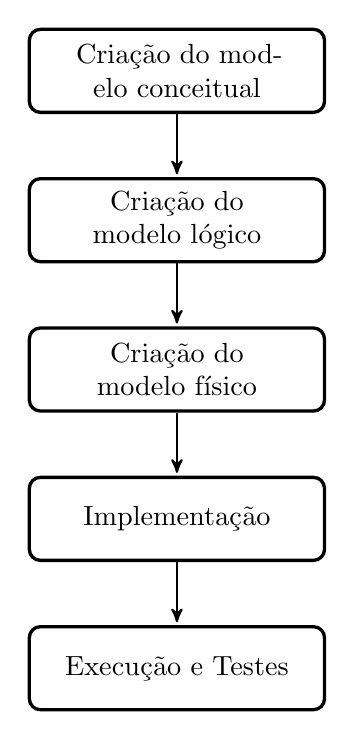
\begin{tikzpicture}
      [node distance=.8cm, start chain=going below,]
         \node[punktchain, join] (etapa1) {Criação do modelo conceitual};
         \node[punktchain, join] (etapa2) {Criação do modelo lógico};
         \node[punktchain, join] (etapa3) {Criação do modelo físico};
         \node[punktchain, join] (etapa4) {Implementação};
         \node[punktchain, join] (etapa5) {Execução e Testes};
    \end{tikzpicture}

    \legend{Fonte: Autor}
    \label{figuramet}
\end{figure}

% ----------------------------------------------------------
% Regras de Negócio
% ----------------------------------------------------------
\chapter {Regras de Negócio}

% ----------------------------------------------------------
% Modelo Conceitual
% ----------------------------------------------------------
\chapter{Modelo Conceitual}
    \begin{figure}[h]
         \centering
         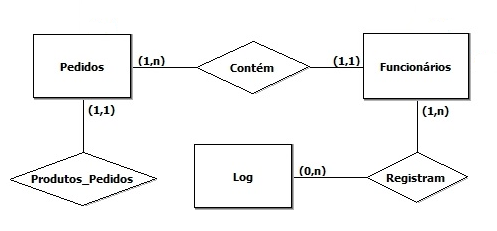
\includegraphics[width=10cm,keepaspectratio]{../BancoDeDadosPizzaria/Imgs/MC_01}
         \caption{ }
         \label{}
    \end{figure}
    
    \begin{figure}[h]
         \centering
         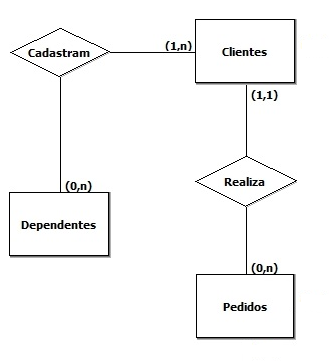
\includegraphics[width=10cm,keepaspectratio]{../BancoDeDadosPizzaria/Imgs/MC_02}
         \caption{ }
         \label{}
    \end{figure}

    \begin{figure}[h]
         \centering
         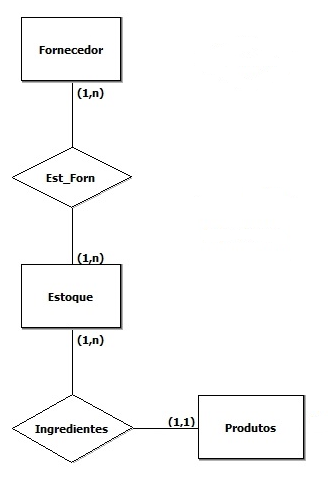
\includegraphics[width=10cm,keepaspectratio]{../BancoDeDadosPizzaria/Imgs/MC_03}
         \caption{ }
         \label{}
    \end{figure}

    \begin{figure}[h]
         \centering
         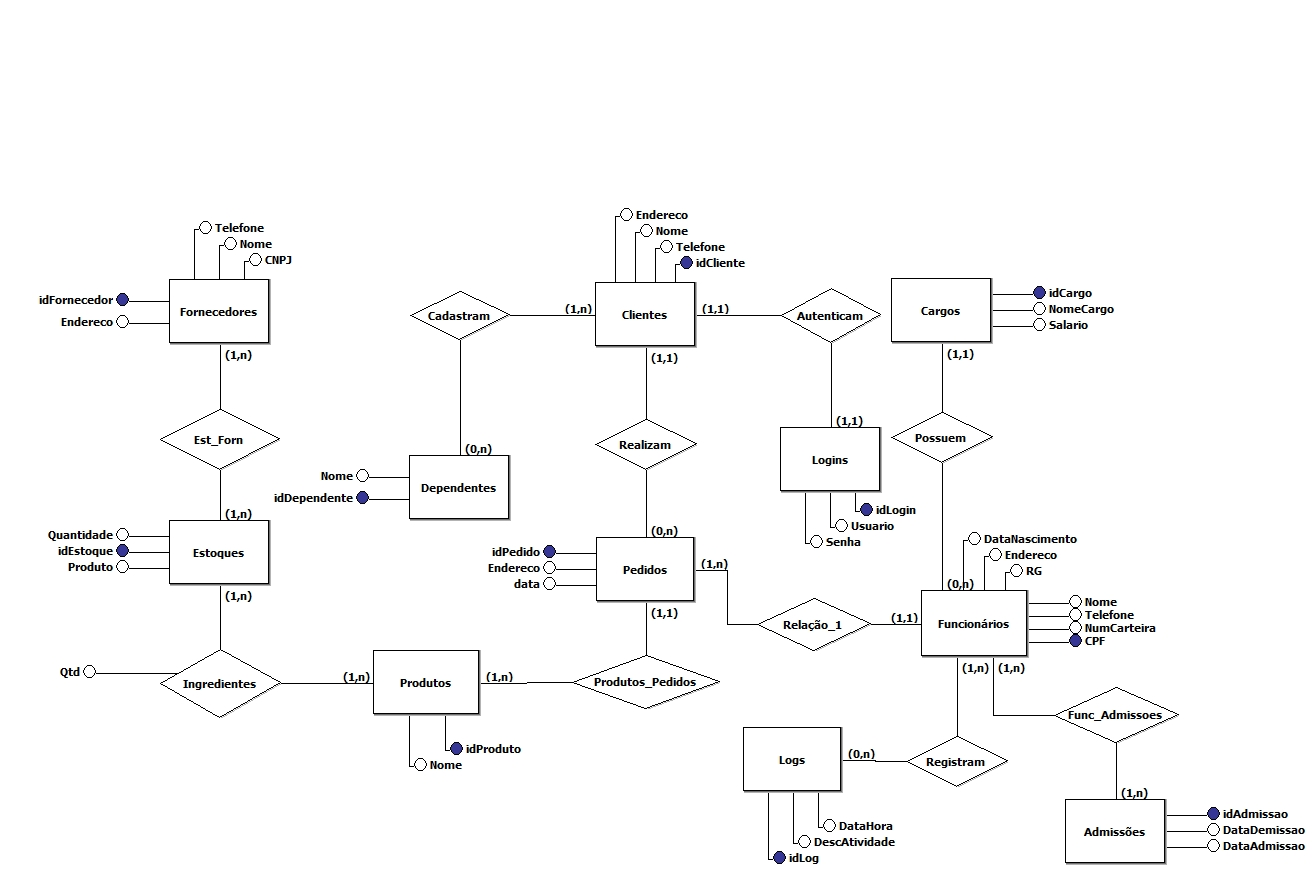
\includegraphics[width=10cm,keepaspectratio,angle=90]{../BancoDeDadosPizzaria/Imgs/MC_00}
         \caption{ }
         \label{}
    \end{figure}    

% ----------------------------------------------------------
% Modelo Lógico
% ----------------------------------------------------------
\chapter{Modelo Lógico}
    \begin{figure}[h]
         \centering
         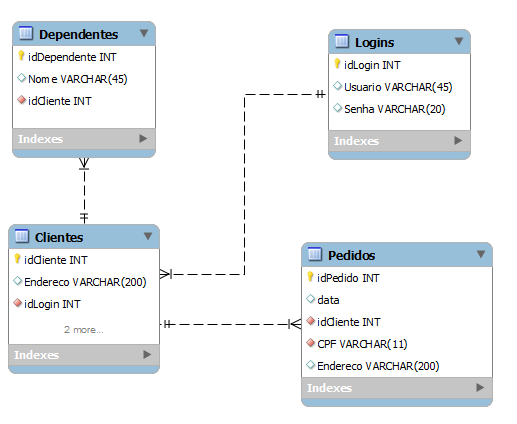
\includegraphics[width=10cm,keepaspectratio]{../BancoDeDadosPizzaria/Imgs/ML_01}
         \caption{ }
         \label{}
    \end{figure}
    
    \begin{figure}[h]
         \centering
         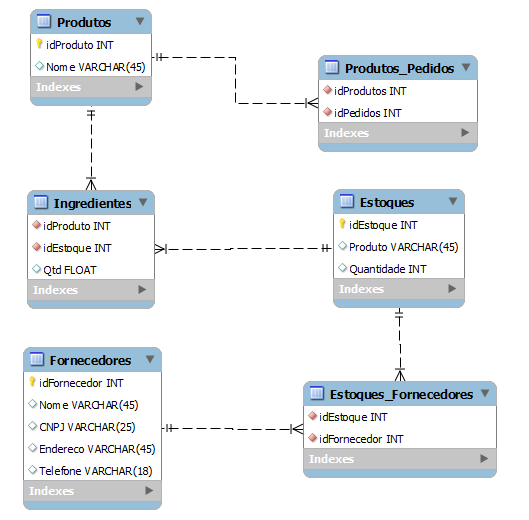
\includegraphics[width=10cm,keepaspectratio]{../BancoDeDadosPizzaria/Imgs/ML_02}
         \caption{ }
         \label{}
    \end{figure}
    
    \begin{figure}[h]
         \centering
         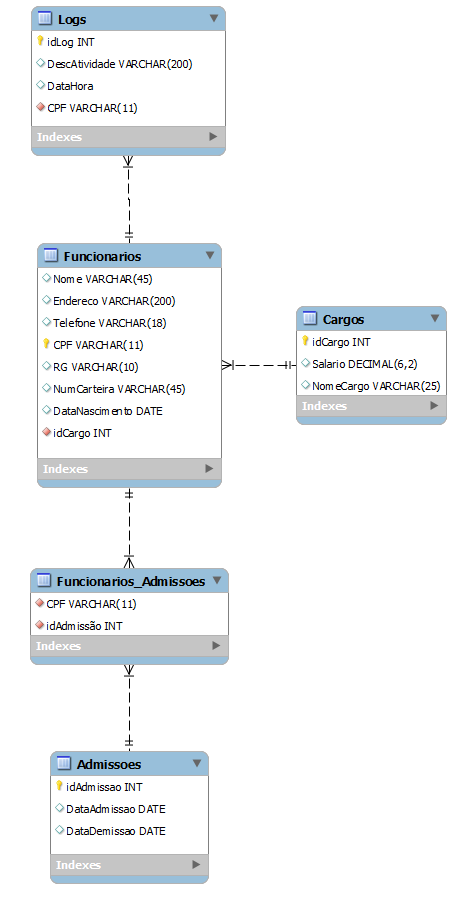
\includegraphics[width=10cm,keepaspectratio]{../BancoDeDadosPizzaria/Imgs/ML_03}
         \caption{ }
         \label{}
    \end{figure}
    
    \begin{figure}[h]
         \centering
         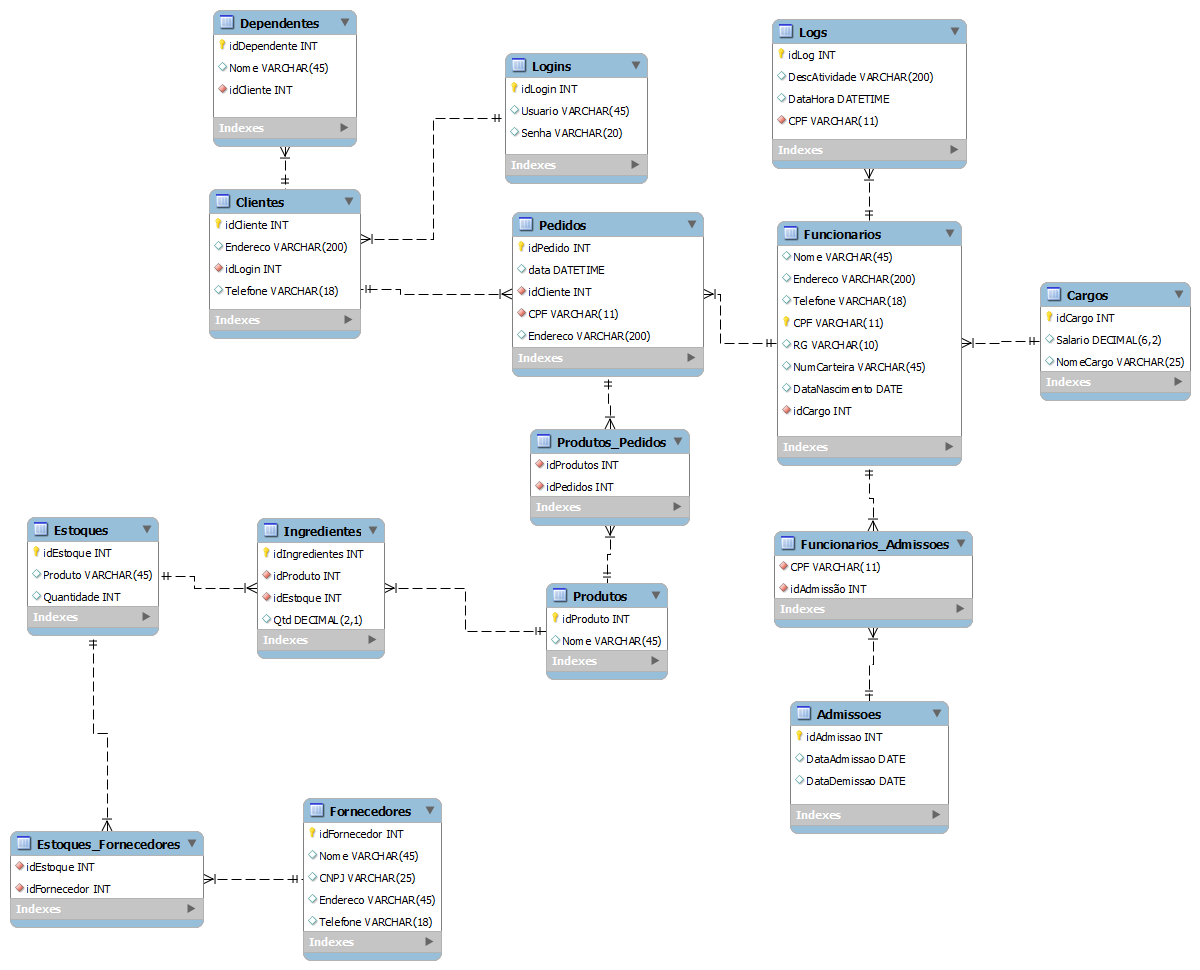
\includegraphics[width=10cm,keepaspectratio, angle=90]{../BancoDeDadosPizzaria/Imgs/ML_00}
         \caption{ }
         \label{}
    \end{figure}

    
% ----------------------------------------------------------
% Implementação
% ----------------------------------------------------------
\chapter{Implementação}
    O banco de dados foi implementado utilizando o \textit{software SQL Server 2010}.
    \lstinputlisting{../BancoDeDadosPizzaria/Sql/ModeloFísico.sql}

% ----------------------------------------------------------
% Execução e Testes
% ----------------------------------------------------------
\chapter {Execução e Testes}
    As execuções e os testes foram feitos utilizando o \textit{software SQL Server Management Studio 2010}.
    
\section{Consultas}
    % Explicar
    \lstinputlisting{../BancoDeDadosPizzaria/Sql/Select_001.sql}
    % Mostrar resultado
    \begin{figure}[h]
         \centering
         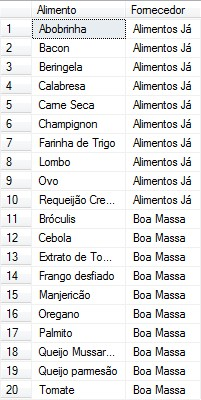
\includegraphics[width=10cm,keepaspectratio]{../BancoDeDadosPizzaria/Imgs/Select_001}
         \caption{Resultado do select}
         \label{}
    \end{figure}
    
    % Explicar
    \lstinputlisting{../BancoDeDadosPizzaria/Sql/Select_002.sql}
    % Mostrar resultado
    \begin{figure}[h]
         \centering
         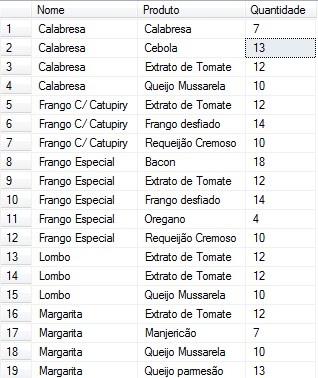
\includegraphics[width=10cm,keepaspectratio]{../BancoDeDadosPizzaria/Imgs/Select_002}
         \caption{Resultado do select}
         \label{}
    \end{figure}
    
    % Explicar
    \lstinputlisting{../BancoDeDadosPizzaria/Sql/Select_003.sql}
    % Mostrar resultado
    \begin{figure}[h]
         \centering
         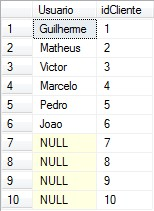
\includegraphics[width=10cm,keepaspectratio]{../BancoDeDadosPizzaria/Imgs/Select_003}
         \caption{Resultado do select}
         \label{}
    \end{figure}
    
    %Explicar
    \lstinputlisting{../BancoDeDadosPizzaria/Sql/Select_004.sql}
    % Mostrar resultado
    \begin{figure}[h]
         \centering
         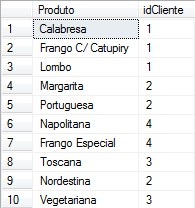
\includegraphics[width=10cm,keepaspectratio]{../BancoDeDadosPizzaria/Imgs/Select_004}
         \caption{Resultado do select}
         \label{}
    \end{figure}
    
    % Explicar
    \lstinputlisting{../BancoDeDadosPizzaria/Sql/Select_005.sql}
    % Mostrar resultado
    \begin{figure}[h]
         \centering
         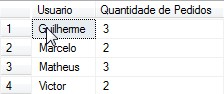
\includegraphics[width=10cm,keepaspectratio]{../BancoDeDadosPizzaria/Imgs/Select_005}
         \caption{Resultado do select}
         \label{}
    \end{figure}
    
    % Explicar
    \lstinputlisting{../BancoDeDadosPizzaria/Sql/Select_006.sql}
    % Mostrar resultado
    \begin{figure}[h]
         \centering
         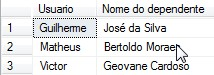
\includegraphics[width=10cm,keepaspectratio]{../BancoDeDadosPizzaria/Imgs/Select_006}
         \caption{Resultado do select}
         \label{}
    \end{figure}

    % Explicar
    \lstinputlisting{../BancoDeDadosPizzaria/Sql/Select_007.sql}
    % Mostrar resultado
    \begin{figure}[h]
         \centering
         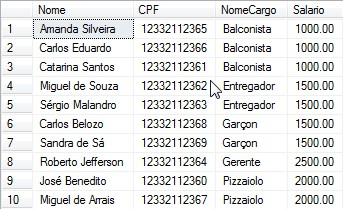
\includegraphics[width=10cm,keepaspectratio]{../BancoDeDadosPizzaria/Imgs/Select_007}
         \caption{Resultado do select}
         \label{}
    \end{figure}    
    
    % Explicar
    \lstinputlisting{../BancoDeDadosPizzaria/Sql/Select_008.sql}
    % Mostrar resultado
    \begin{figure}[h]
         \centering
         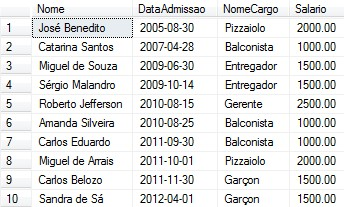
\includegraphics[width=10cm,keepaspectratio]{../BancoDeDadosPizzaria/Imgs/Select_008}
         \caption{Resultado do select}
         \label{}
    \end{figure}
       
\section{Procedimentos armazenados}

    % Explicar
    \lstinputlisting{../BancoDeDadosPizzaria/Sql/USP_001.sql}
    % Mostrar resultado
    \begin{figure}[h]
         \centering
         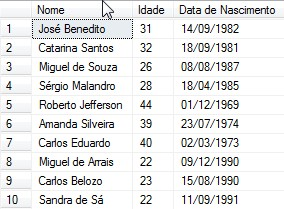
\includegraphics[width=10cm,keepaspectratio]{../BancoDeDadosPizzaria/Imgs/USP_001}
         \caption{Resultado do select}
         \label{}
    \end{figure}
    
    % Explicar
    \lstinputlisting{../BancoDeDadosPizzaria/Sql/USP_002.sql}
    % Mostrar resultado
    \begin{figure}[h]
         \centering
         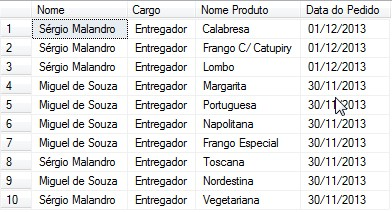
\includegraphics[width=10cm,keepaspectratio]{../BancoDeDadosPizzaria/Imgs/USP_002}
         \caption{Resultado do select}
         \label{}
    \end{figure}
    
    % Explicar
    \lstinputlisting{../BancoDeDadosPizzaria/Sql/USP_003.sql}
    % Mostrar resultado
    \begin{figure}[h]
         \centering
         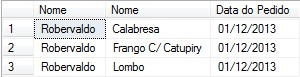
\includegraphics[width=10cm,keepaspectratio]{../BancoDeDadosPizzaria/Imgs/USP_003p1}
         \caption{Resultado do select}
         \label{}
    \end{figure}
    
    \begin{figure}[h]
         \centering
         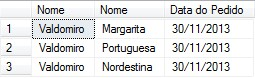
\includegraphics[width=10cm,keepaspectratio]{../BancoDeDadosPizzaria/Imgs/USP_003p2}
         \caption{Resultado do select}
         \label{}
    \end{figure}

% ---
% Finaliza a parte no bookmark do PDF
% para que se inicie o bookmark na raiz
% e adiciona espaço de parte no Sumário
% ---
\phantompart

% ---
% Conclusão
% ---
\chapter*[Considerações]{Considerações Finais}
\addcontentsline{toc}{chapter}{Considerações Finais}

Apesar de parecer simples, criar um banco de dados para uma pizzaria mostrou-se 
uma tarefa cheia de detalhes a se pensar. Ao ser implementado, tornou-se 
funcional, sendo possível utilizá-lo em um ambiente real.

% ----------------------------------------------------------
% ELEMENTOS PÓS-TEXTUAIS
% ----------------------------------------------------------
\postextual

% ----------------------------------------------------------
% Referências bibliográficas
% ----------------------------------------------------------
% \bibliography{abntex2-modelo-references}
\bibliography{ref}

% ----------------------------------------------------------
% Glossário
% ----------------------------------------------------------
%
% Consulte o manual da classe abntex2 para orientações sobre o glossário.
%
%\glossary

% ----------------------------------------------------------
% Apêndices
% ----------------------------------------------------------

% ---
% Inicia os apêndices
% ---
% \begin{apendicesenv}

% % Imprime uma página indicando o início dos apêndices
% \partapendices

% % ----------------------------------------------------------
% \chapter{Quisque libero justo}
% % ----------------------------------------------------------

% \lipsum[50]

% % ----------------------------------------------------------
% \chapter{Nullam elementum urna vel imperdiet sodales elit ipsum pharetra ligula
% ac pretium ante justo a nulla curabitur tristique arcu eu metus}
% % ----------------------------------------------------------
% \lipsum[55-57]

% \end{apendicesenv}
% ---


% ----------------------------------------------------------
% Anexos
% ----------------------------------------------------------

% ---
% Inicia os anexos
% ---
\begin{anexosenv}

% % Imprime uma página indicando o início dos anexos
\partanexos

% % ---
\chapter{Dados inseridos para teste}
% % ---
\lipsum[30]

\lstinputlisting{../BancoDeDadosPizzaria/Sql/Inserts.sql}

\end{anexosenv}

%---------------------------------------------------------------------
% INDICE REMISSIVO
%---------------------------------------------------------------------

\phantompart
\printindex

\end{document}